\section{iQAN: Fast and Accurate ANNS via Intra-Query Parallelism on Multi-Core Architecture}
\label{minjia_sec:iqan}

Among different vector search methods, the similarity graph-based algorithms have emerged as a remarkably effective class of methods for high-dimensional ANNS, outperforming other approaches on a wide range of datasets to achieve the best accuracy-vs-latency~\cite{nsg,ann-benchmark,li2020approximate,echihabi2019return,wei2020analyticdb,wang2020deltapq,product-quantization,babenko2014inverted}. Despite their promising results, graph-based methods still have challenges that limit their use in real-world scenarios.
In particular, as the data size grows, it becomes increasingly challenging to achieve both low latency and high accuracy simultaneously. Existing solutions often resort to inter-query parallelism by dispatching queries across multiple processors or nodes to be processed simultaneously~\cite{nsg,bashyam2020fast}. This approach scales from a throughput perspective, but it does not help reduce query latency because each query still roughly performs the same amount of vector computations to find the nearest neighbors.

\subsection{Challenges of ANNS via Intra-Query Parallelism}

Another natural idea to reduce latency is to exploit intra-query parallelism on individual nodes with multi-core processors. For example, one may parallelize the node expansion in each iteration step of the sequential search algorithm (referred to as \textbf{Node-Expansion-in-Parallel}) because distance computations within a neighborhood expansion iteration do not have dependencies, hoping that multiple worker threads can check the closeness of multiple neighbors in parallel while performing the same computations on each step as the sequential algorithm.  Surprisingly, this solution performs quite poorly and may even perform much worse than a well-tuned sequential algorithm, as shown in Fig.~\ref{minjia_fig:insight_edge_wise_latency}. There are several challenges in scaling ANNS with intra-query parallelism:

\textbf{Challenge 1: Modern multi-core hardware is sensitive to synchronization overhead.}
Parallelism boosts compute capacity but may also incur high synchronization overhead, especially if there are complex data dependencies. While parallelizing the distance computation,  Node-Expansion-in-Parallel also requires synchronization in between expansion iterations to sort the distance order of all candidates discovered by multiple parallel workers according to their distances to the query point, to decide which node to expand in the next iteration. We have observed that the synchronization is very expensive on a multi-core architecture, and frequent sequential-to-parallel synchronization as in Node-Expansion-in-Parallel can significantly prolong the search process. 
Fig.~\ref{minjia_fig:insight_edge_wise_sync_overhead} shows that as we increase the number of threads, the synchronization overhead accounts for more than 50\%
of the total search time, becoming a dominating factor in the overall search latency. 

\begin{figure}[!ht]
\begin{minipage}[t]{0.23\textwidth}
    \centering
    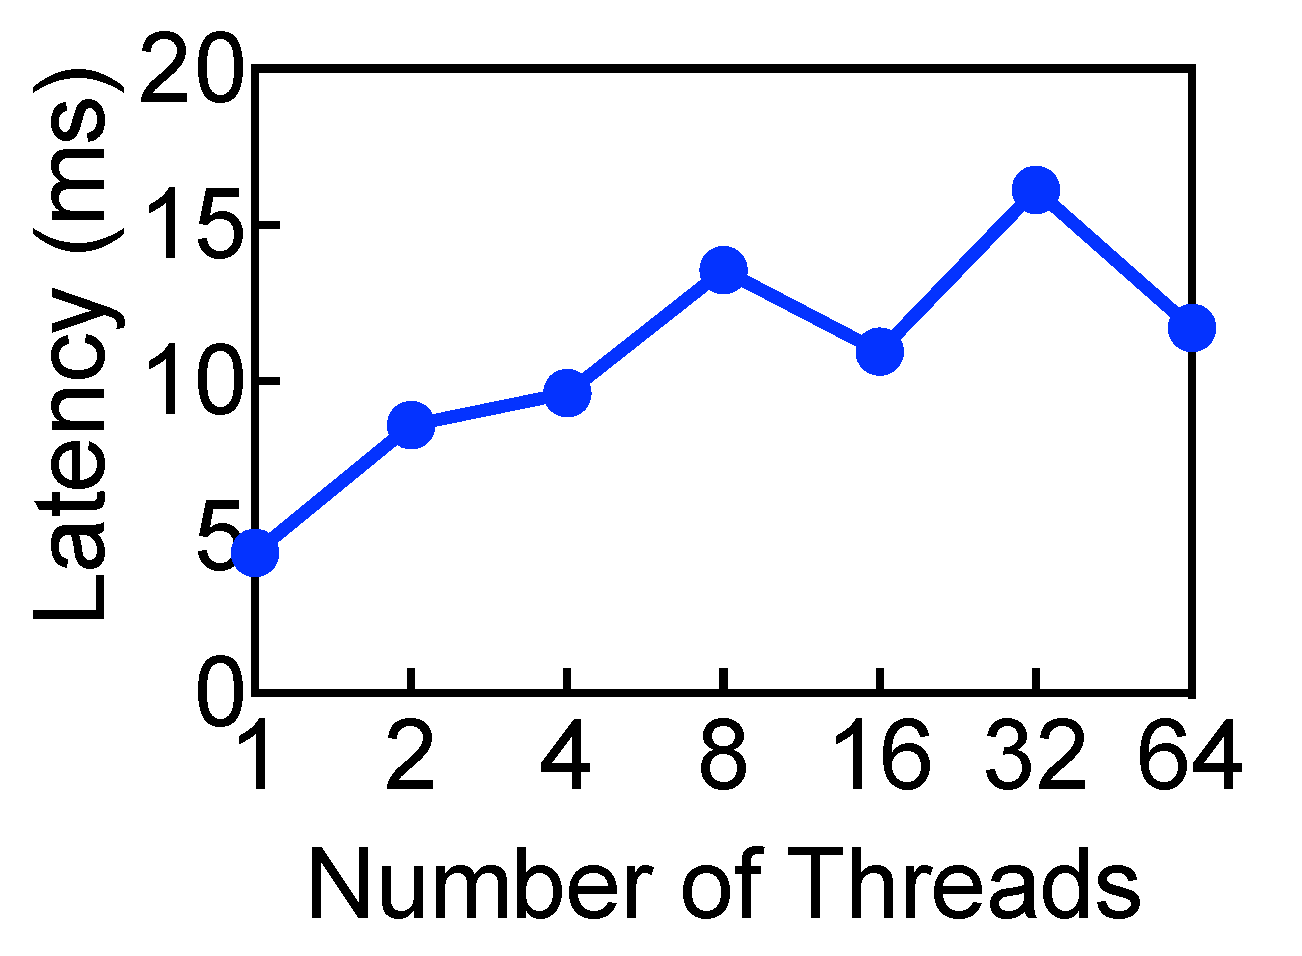
\includegraphics[height=0.98in]{submissions/Minjia2023/figures/insight_edge_wise_latency.pdf}
    \caption{
        {EP's latency on Deep100M.}
    }
    \label{minjia_fig:insight_edge_wise_latency}
\end{minipage}
\hfill
\begin{minipage}[t]{0.23\textwidth}
    \centering
    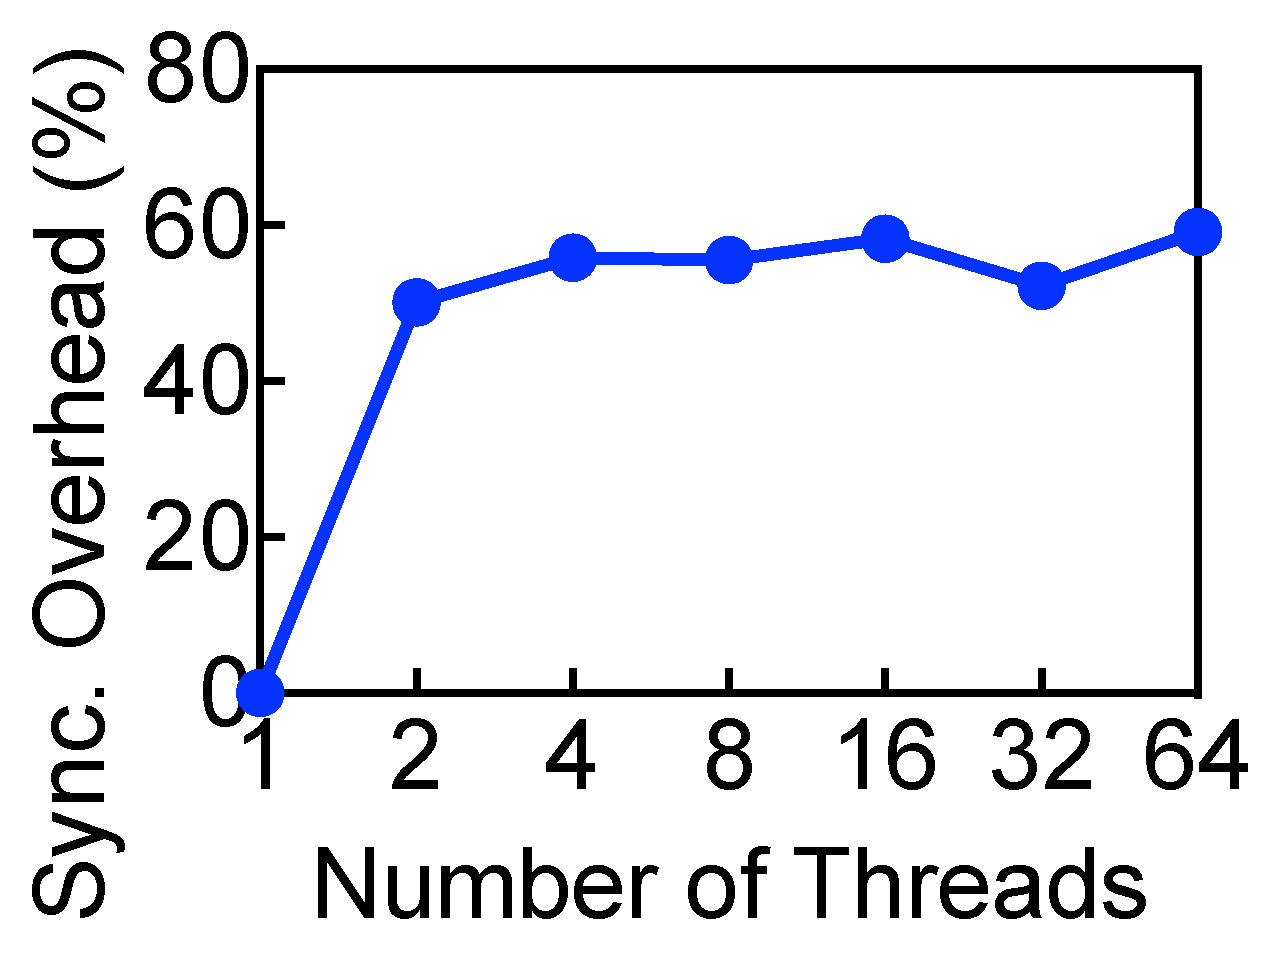
\includegraphics[height=0.98in]{submissions/Minjia2023/figures/insight_edge_wise_sync_overhead}
    \caption{
        {EP adds high sync. overhead.}
    }
    \label{minjia_fig:insight_edge_wise_sync_overhead}
\end{minipage}
\hfill
\begin{minipage}[t]{0.23\textwidth}
    \centering
    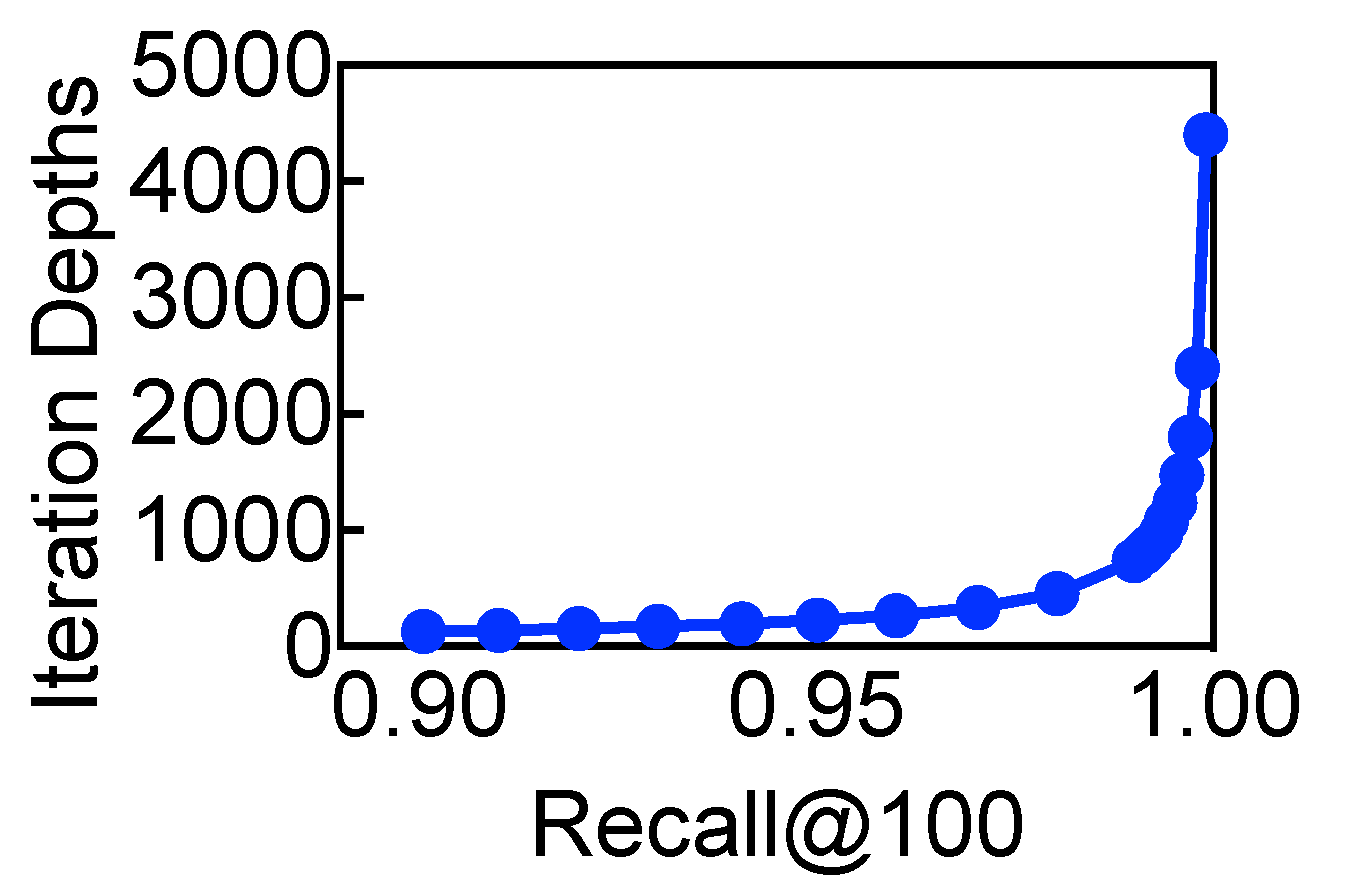
\includegraphics[height=0.9in]{submissions/Minjia2023/figures/insight_NSG_convergence_vs_recall}
    \caption{
        {Iteration depths change along with recall.}
    }
    \label{minjia_fig:insight_NSG_convergence_vs_recall}
\end{minipage}
\hfill
\begin{minipage}[t]{0.23\textwidth}
    \centering
    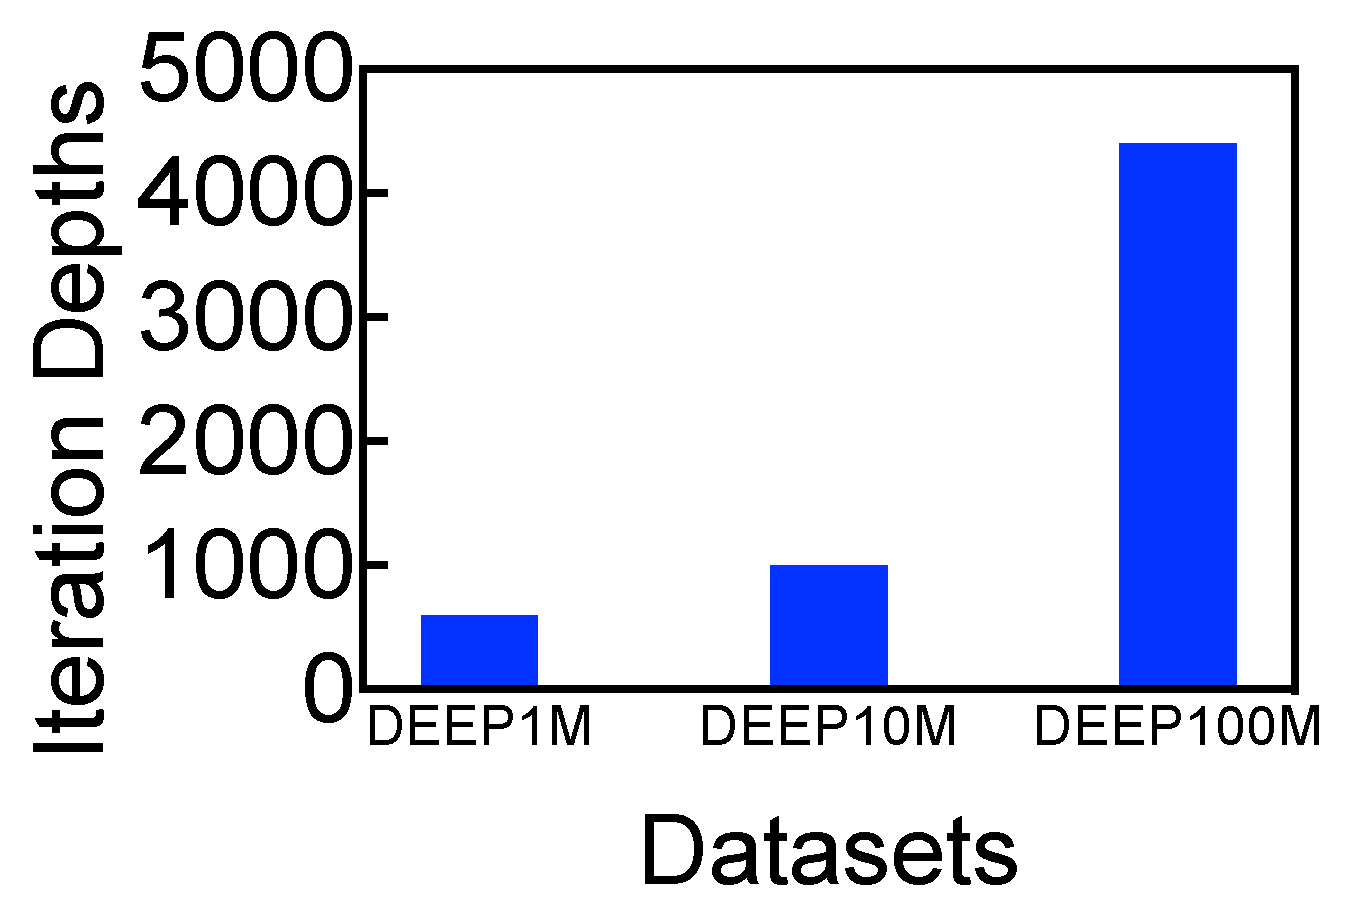
\includegraphics[height=0.9in]{submissions/Minjia2023/figures/insight_NSG_convergence_vs_dataset_sizes}
    \caption{
        {Iteration depths change along with data sizes.}
    }
    \label{minjia_fig:insight_NSG_convergence_vs_dataset_sizes}
\end{minipage}
\end{figure}

\textbf{Challenge 2: Node-Expansion-in-Parallel leads to insufficient computation granularity per worker, leading to sub-optimal memory bandwidth utilization.} Node-Expansion-in-Parallel has low compute intensity because (1) unlike matrix multiplication, the point-wise Euclidean distance computation is an operator with low compute intensity, and (2) the number of neighbors to be expanded in one step is limited, given that similarity graphs naturally have low out-degree to avoid the \emph{out-degree explosion problem}~\cite{nsg}. As such, further dividing the distance computation within each neighbor expansion iteration leads to insufficient work for each worker. 

\textbf{Challenge 3: Vector search using graph traversal requires many iterations to converge, resulting in long sequential dependencies between iterations and thus limiting its scalability.}
The number of neighborhood expansion iterations depends on the recall target and the graph size. For example, 
Fig.~\ref{minjia_fig:insight_NSG_convergence_vs_recall} shows that as the recall target increases, the number of iterations to find the top-100 nearest neighbors on a hundred million scale dataset {DEEP100M} grows dramatically as the recall target becomes higher (e.g., a $34.6$-time increase from 0.9 to 0.999 recall). 
Fig.~\ref{minjia_fig:insight_NSG_convergence_vs_dataset_sizes} shows that as the dataset size increases, the number of iterations to find the results for recall target 0.999 also grows  (e.g., $7.3$ times from 1M-vector dataset to 100M-vector dataset). This long sequential dependency makes achieving low latency with high accuracy especially challenging. 

\subsection{Design of \Hammer}
\label{minjia_subsec:iqan-design}

To address the aforementioned challenges, we introduce \Hammer, a parallel search algorithm to accelerate graph-based ANNS on multi-core architectures with three key optimizations: (i) reducing neighbor expansion iteration depth by path-wise parallelism, (ii) reducing redundant distance computation by staged expansion, and (iii) reducing synchronization overhead by redundancy-aware synchronization. 

\subsubsection{Reduce Iteration Depth by Intra-Query Path-Wise Parallelism} 
\label{minjia_subsec:path-wise}


In each search iteration, a Best-First-Search (\SeqShortName) algorithm is often used to perform node expansion to the most promising unchecked candidate~\cite{hnsw,nsg}. In \Hammer, we make a small modification to this process by relaxing the priority order and letting each thread expand a few more nodes (e.g., top $W$ unchecked candidates) in every step as active nodes for expansion. We also relax the synchronization such that a global synchronization is only performed after a few expansion steps. We call this new way of expanding nodes \emph{path-wise parallelism (PP)}. This small change in algorithm results in a significant reduction in iteration depths for queries, e.g., from a few {thousands} to {tens} in some cases.

Why would this change reduce the iteration depth? The multi-node expansion and relaxed synchronizations are equivalent to letting each thread explore paths in a local region instead of a single node's neighbor list before doing a global synchronization. By doing so, it increases the likelihood of finding nearest neighbors in less number of iterations. 
Fig.~\ref{minjia_fig:insight_convergence_steps_Top_M_vs_SGS} shows the comparison results of iteration depths between \SeqShortName and \emph{PP} on dataset SIFT1M using 10K queries with a $0.90$ recall target. We set $W$ to 64. Overall, while \SeqShortName takes 10.1, 69.4, and 88.1 steps to find the top-1, top-50, and top-100 near neighbor, \emph{PP} only takes 3.4, 5.0, and 5.4 steps on average, respectively, a significant reduction. From the unchecked node's perspective, Fig.~\ref{minjia_subfig:insight_unchecked_vs_iters} shows that \emph{PP} also takes much fewer steps to converge to a local optimum (i.e., finish examining all the unchecked vertices) than \SeqShortName. 

\begin{figure}[t]
    \begin{minipage}[t]{0.23\textwidth}
        \centering
        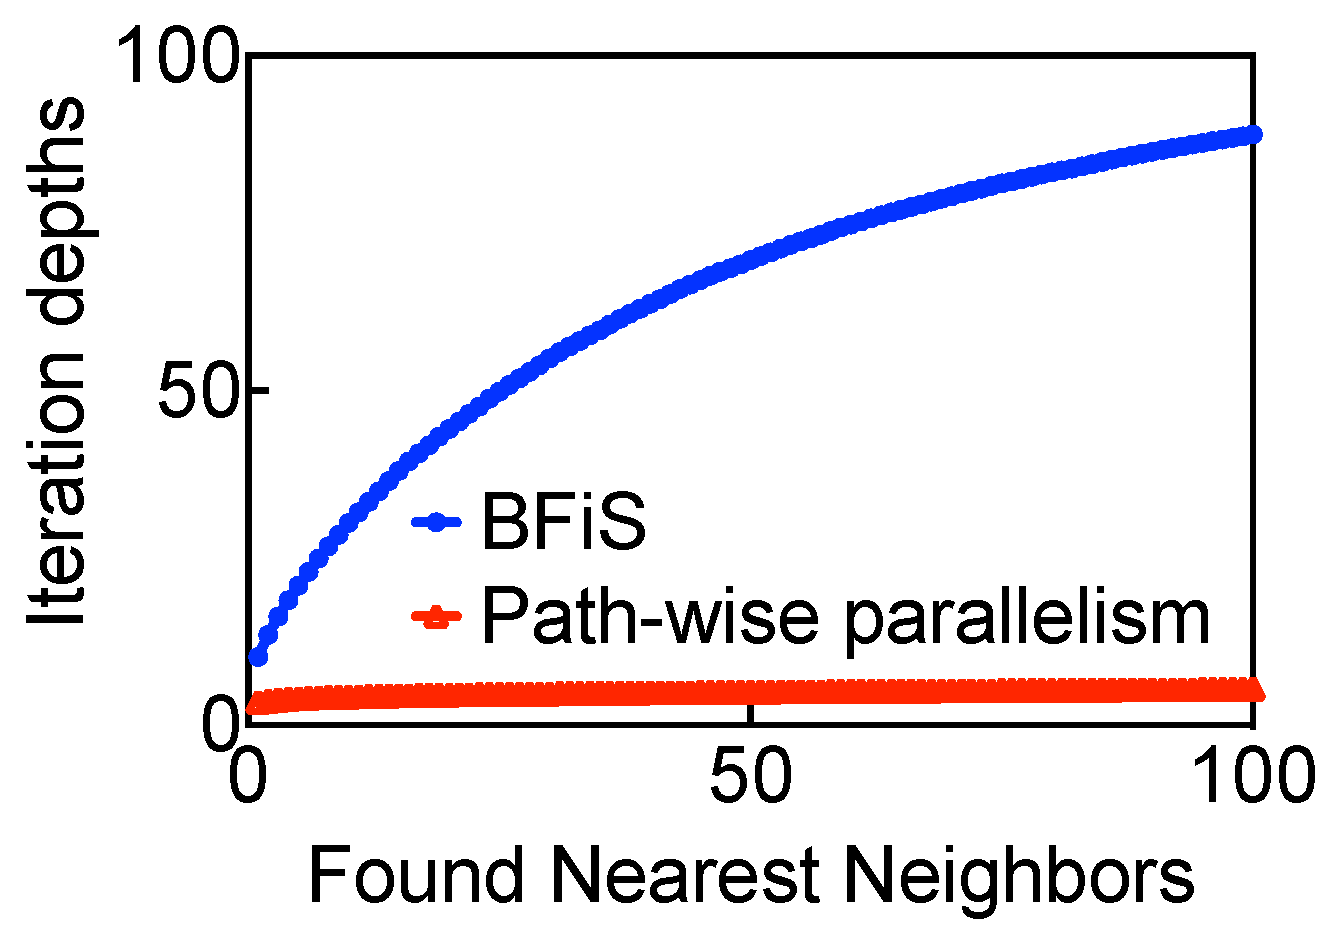
\includegraphics[height=0.9in]{submissions/Minjia2023/figures/insight_last_update_iter_vs_rank}
        \caption{Iteration depths to find the $K$-th nearest neighbor (x-axis).}
        \label{minjia_fig:insight_convergence_steps_Top_M_vs_SGS}
    \end{minipage}
    \hfill
    \begin{minipage}[t]{0.23\textwidth}
        \centering
        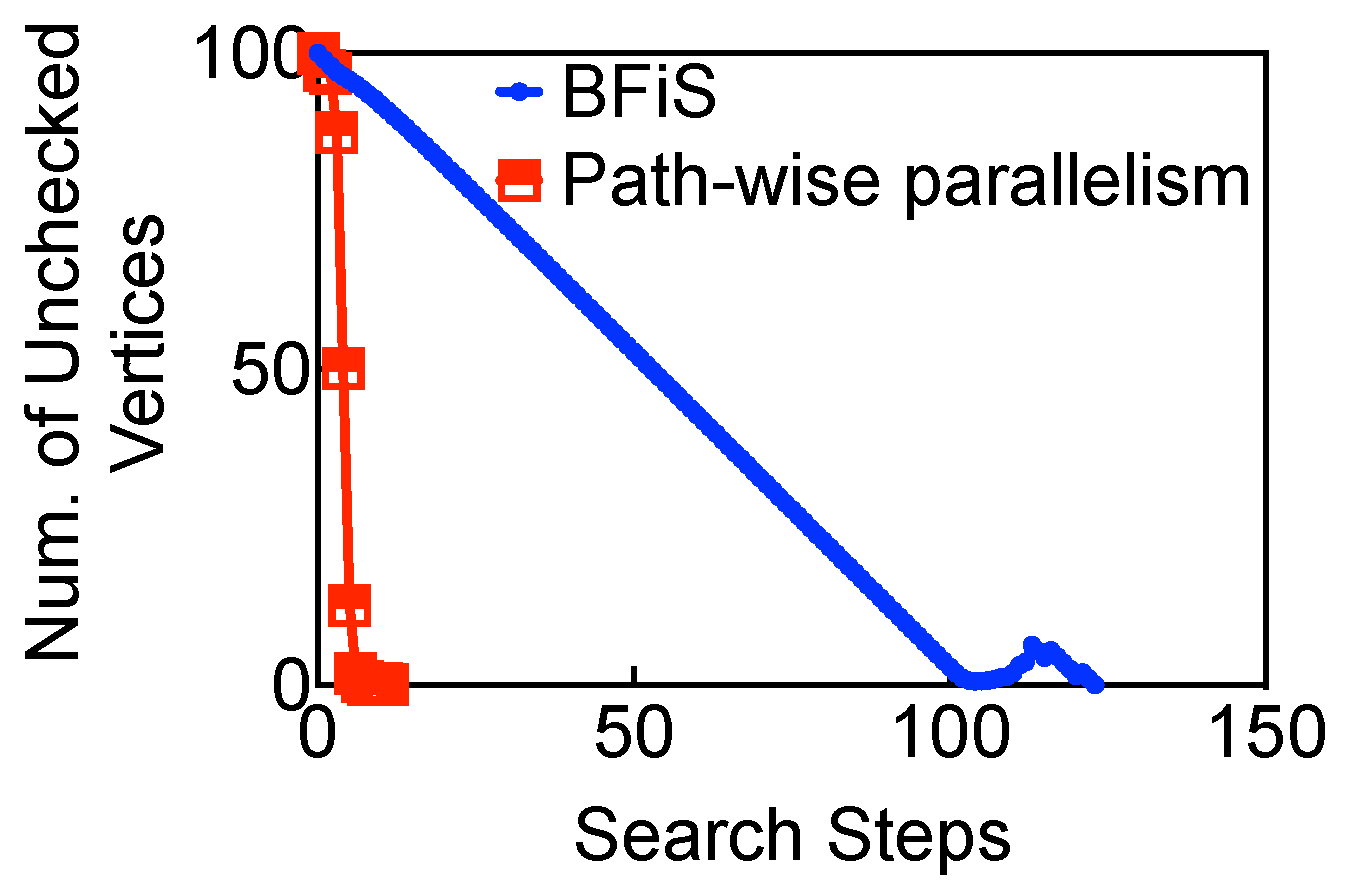
\includegraphics[height=0.9in]{submissions/Minjia2023/figures/insight_unchecked_vs_iters}
        \caption{The number of steps for a search to converge.}
        \label{minjia_subfig:insight_unchecked_vs_iters}
    \end{minipage}
        \hfill
    \begin{minipage}[t]{0.23\textwidth}
        \centering
        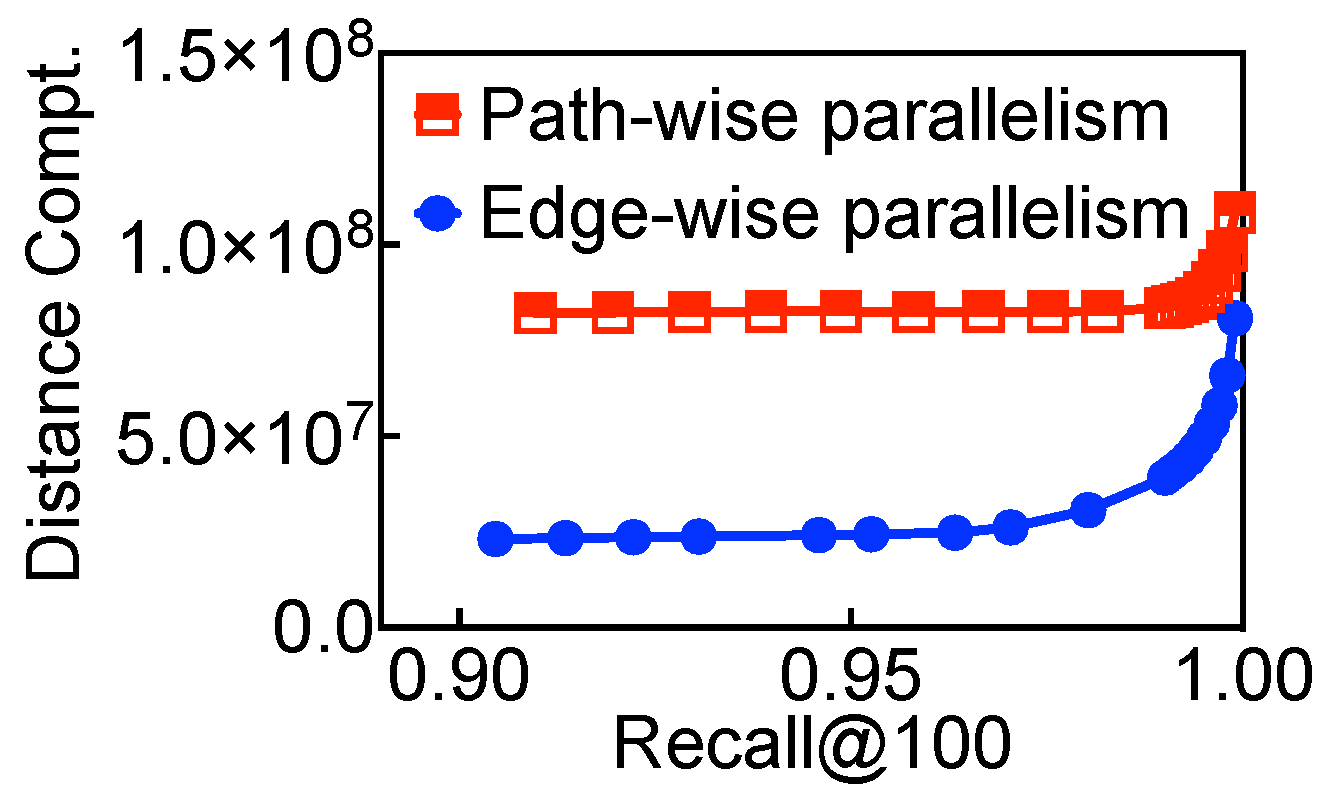
\includegraphics[height=0.90in]{submissions/Minjia2023/figures/insight_1T_compt_Top_M_vs_SGS}
        \caption{
            {Aggregated distance computations of \SeqShortName w/ EP and PP, where $W = 64$.}}
        \label{minjia_fig:insight_1T_compt_Top_M_vs_SGS}
    \end{minipage}
    \hfill
    \begin{minipage}[t]{0.23\textwidth}
        \centering
        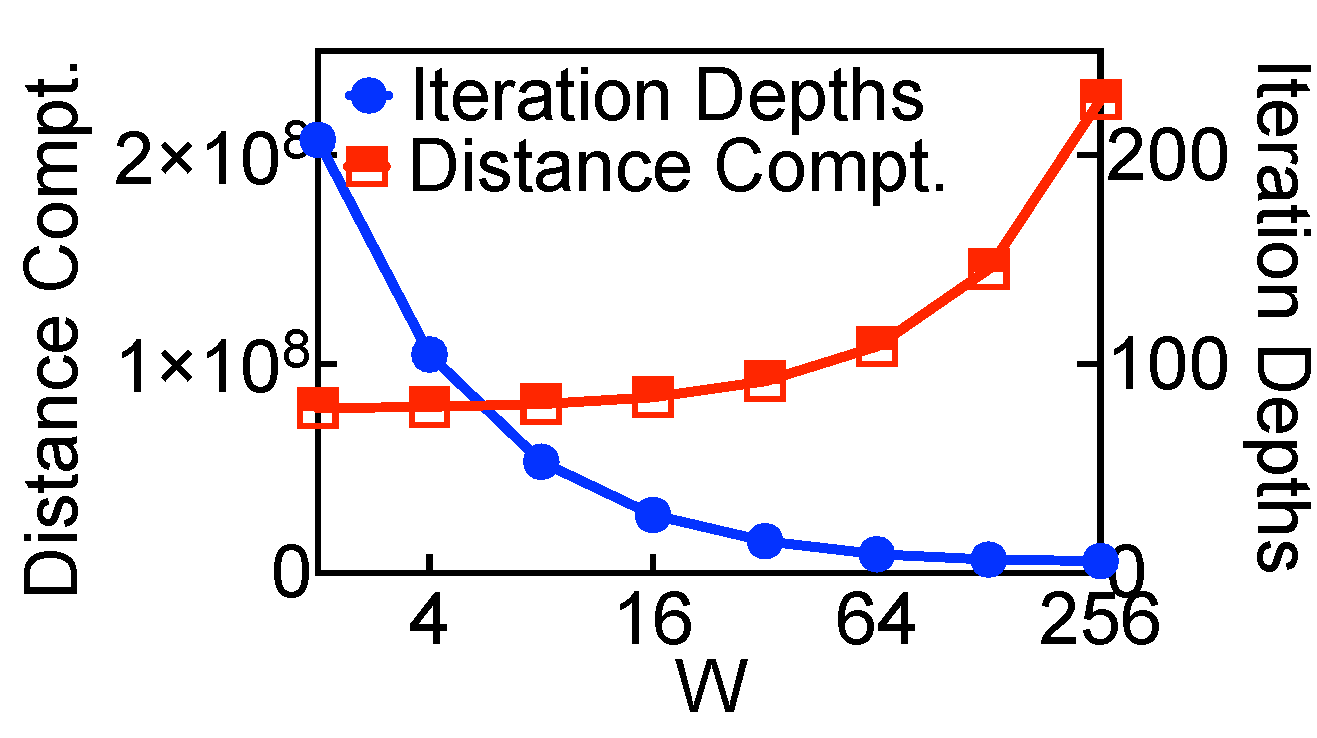
\includegraphics[height=0.90in]{submissions/Minjia2023/figures/insight_Top_M_compt_steps_vs_M}
        \caption{
            Dist. compt. increases as iter. depths decrease for PP increasing $W$.}
        \label{minjia_fig:insight_Top_M_compt_steps_vs_M}
    \end{minipage}
\end{figure}

\subsubsection{Reduce Redundant Computation by Staged Expansion}
\label{minjia_subsec:staged-expansion}

Although reducing the iteration depth significantly, does it mean the search process will now get desired speedups on multi-core architectures? The answer is no. The path-wise parallelism reduces iteration depths but at the same time introduces a considerate amount of additional distance computations, especially when the number of parallel workers is large. 
Fig.~\ref{minjia_fig:insight_1T_compt_Top_M_vs_SGS} shows that to reach the same recall (0.9--0.999), the path-wise parallelism often needs to perform significantly more distance computations than \SeqShortName (1.3--3.5 times). Moreover, we also observe that although the iteration depths continue to decrease by increasing the concurrent expansion width $W$, the number of distance computations inversely increases, as shown in Fig.~\ref{minjia_fig:insight_Top_M_compt_steps_vs_M}. 
The huge amount of redundant computations adversely affects search efficiency as many threads are loading vectors for unnecessary computations, wasting memory bandwidth and compute resources. 

To mitigate it, we investigate the usefulness of path-wise parallelism at different search stages: at which stage does the path-wise parallelism reduce the iteration depths the most? 
We found that overall, in the beginning, since all candidates are far from the query, those early expanded candidates are likely to be discarded by closer ones that are visited later. In other words, candidates expanded and checked at an earlier stage have a high likelihood of becoming unnecessary from a future perspective. As the search moves forward toward the region that has near neighbors, a larger expansion width that covers more search paths can effectively prevent the search from getting stuck at a local minimum.

\begin{figure}[t]
\begin{minipage}[t]{0.23\textwidth}
    \centering
    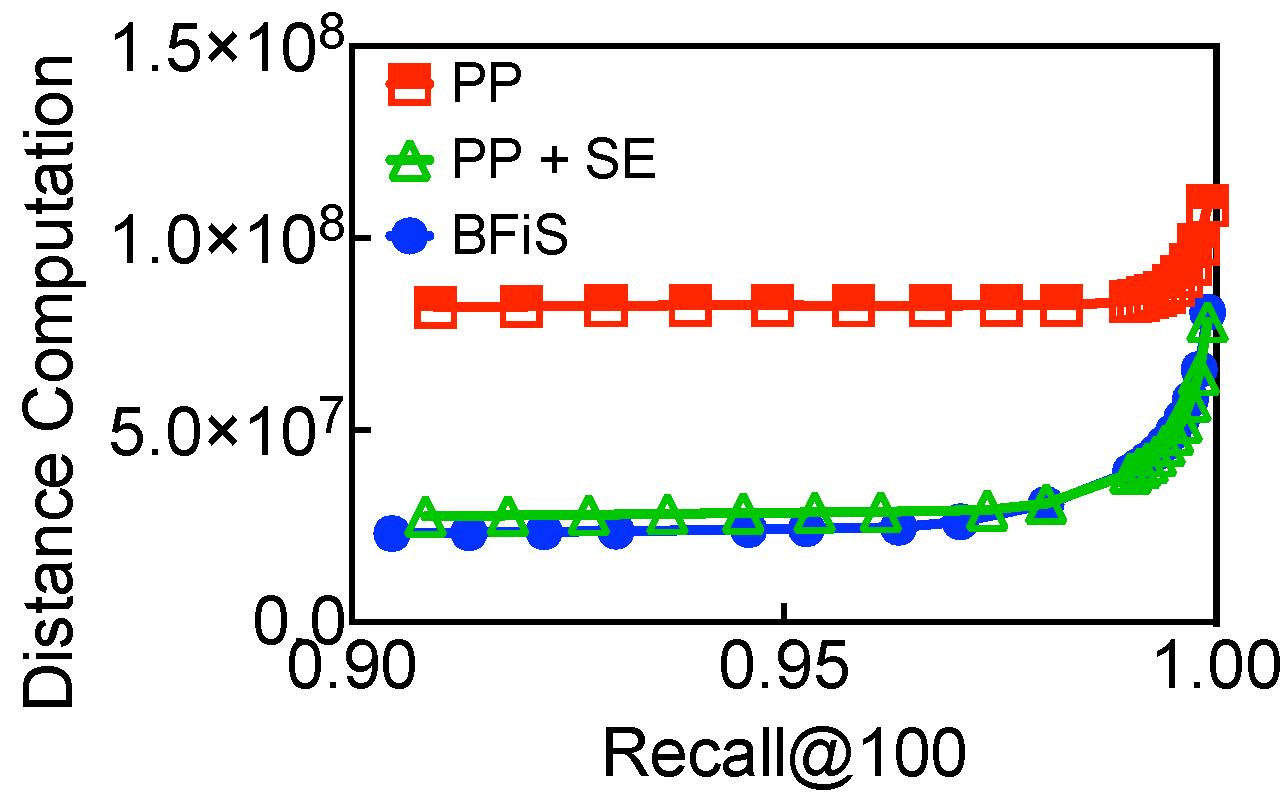
\includegraphics[height=0.91in]{submissions/Minjia2023/figures/insight_1T_compt_Scale_M_vs_Top_M_vs_SGS}
    \caption{Dist. computation of \SeqShortName, PP w/o and w/ staged expansion.}
    \label{minjia_subfig:insight_1T_compt_Scale_M_vs_Top_M_vs_SGS}
\end{minipage}
\hfill
\begin{minipage}[t]{0.23\textwidth}
    \centering
    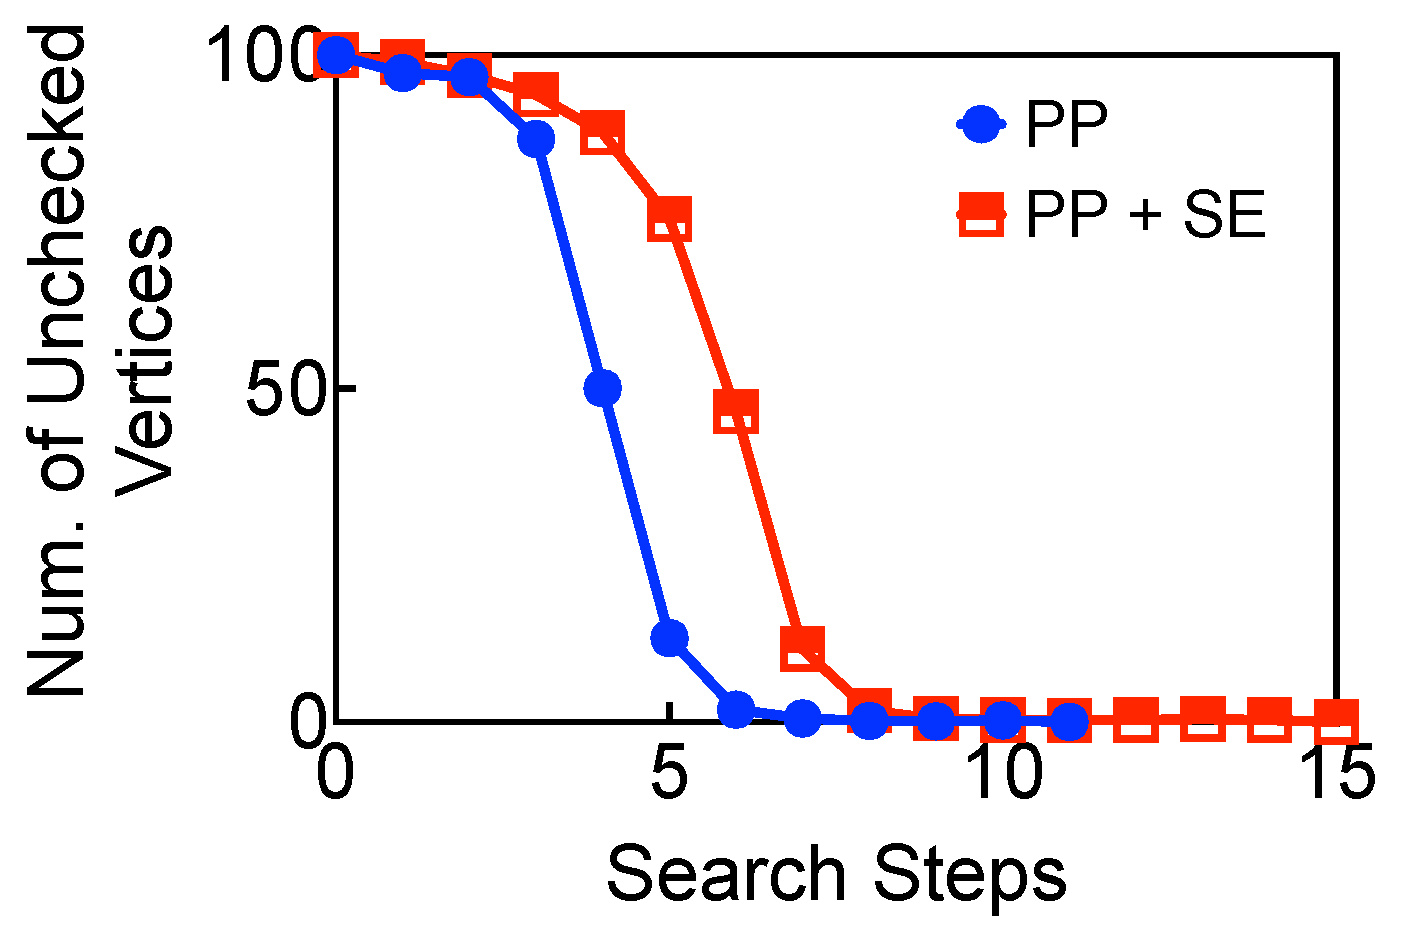
\includegraphics[height=0.91in]{submissions/Minjia2023/figures/insight_unchecked_vs_iter_Top_M_Scale_M}
    \caption{Number of unchecked candidates after each search step. }
    \label{minjia_subfig:insight_unchecked_vs_iter_Top_M_Scale_M}
\end{minipage}
\hfill
    \begin{minipage}[t]{0.23\textwidth}
        \centering
        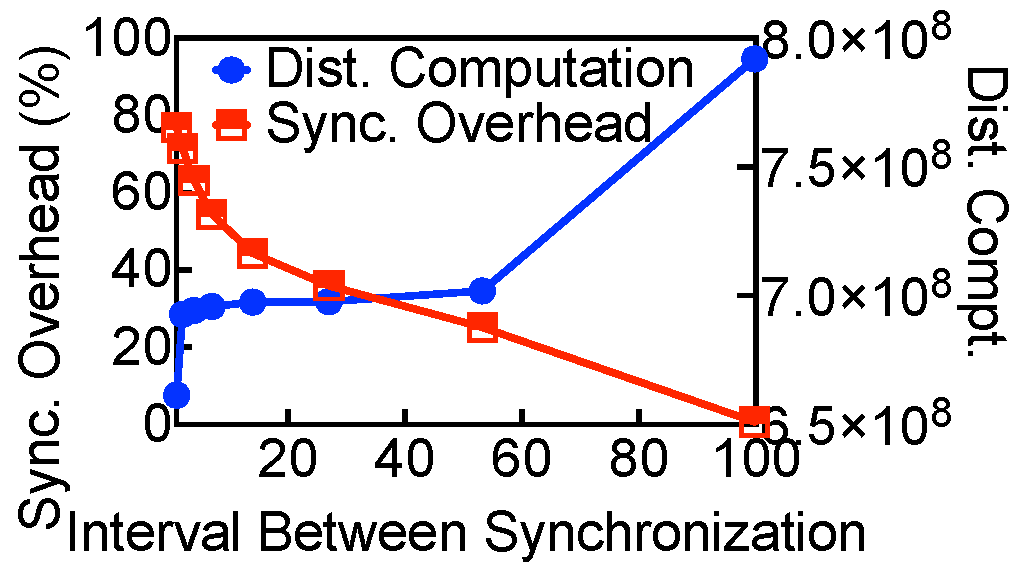
\includegraphics[height=0.97in]{submissions/Minjia2023/figures/insight_PSS_sync_interval_vs_overhead}
        \caption{
            {Sync. overhead and distance compt. as the sync. interval increases.}}
        \label{minjia_fig:insight_PSS_sync_interval_vs_overhead}
    \end{minipage}
    \hfill
    \begin{minipage}[t]{0.23\textwidth}
        \centering
        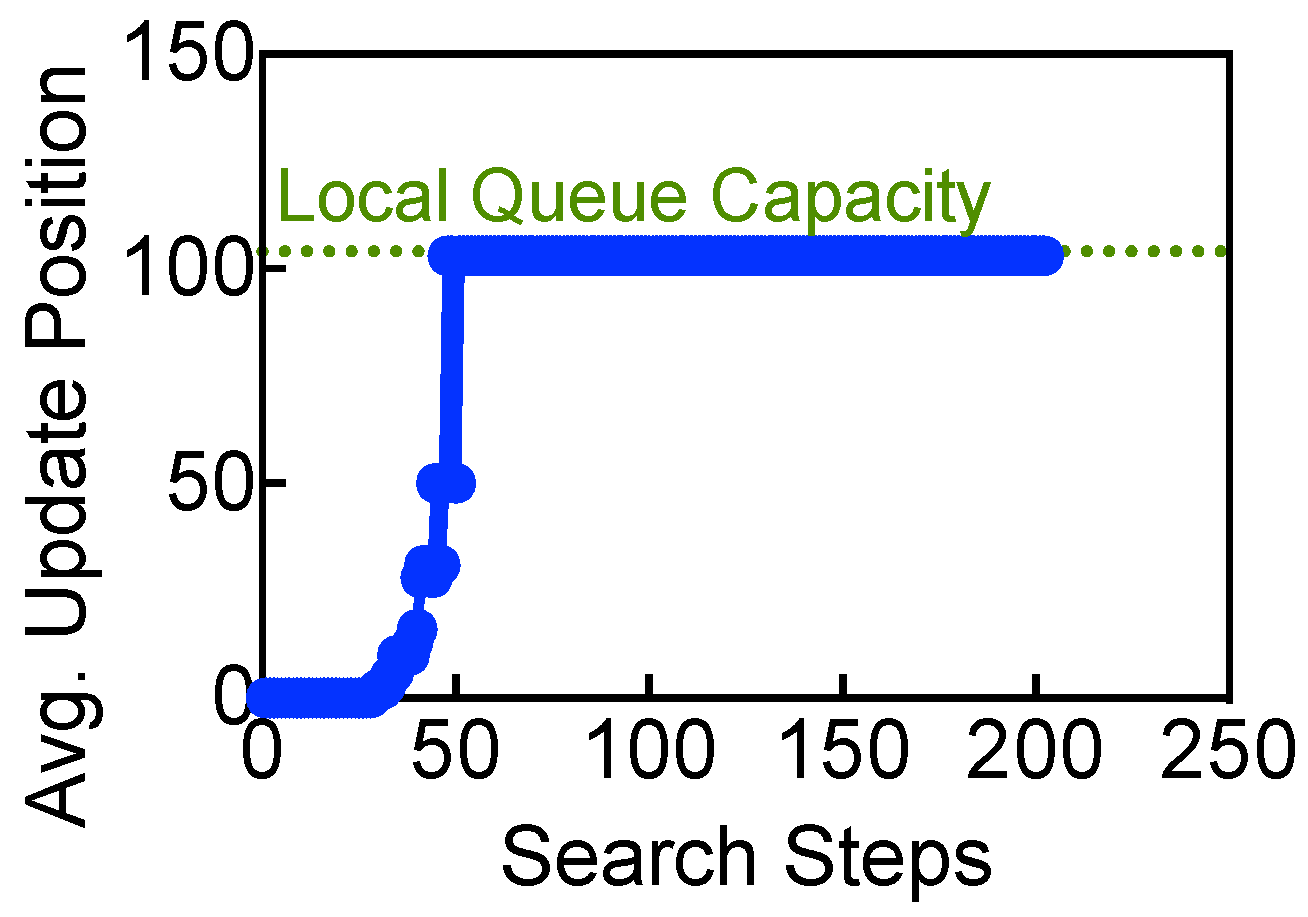
\includegraphics[height=0.97in]{submissions/Minjia2023/figures/insight_PSS_update_position_example}
        \caption{A query's average update positions during searching.
        }
        \label{minjia_fig:insight_PSS_update_position_example}
    \end{minipage}
\end{figure}

Based on these observations, we propose a \emph{staged expansion (SE)} scheme by gradually increasing the expansion width $W$ and the number of workers every $t$ steps during the search procedure. In practice, we set the starting value of $W$ to 1 and the maximum value as the number of available hardware threads. Then for every $t$ steps (e.g., $t=1$) we double the value of $W$ until $W$ reaches its maximum. Fig.~\ref{minjia_subfig:insight_1T_compt_Scale_M_vs_Top_M_vs_SGS} shows the comparison results of path-wise parallelism without and with staged expansion. The staged expansion reduces the number of redundant distance computations significantly, leading to distance computations comparable to \SeqShortName. On the other hand, staged expansion is able to preserve the benefits of path-wise parallelism in terms of obtaining reduced iteration depths, as shown in Fig.~\ref{minjia_subfig:insight_unchecked_vs_iter_Top_M_Scale_M}. These results indicate that by performing path-wise parallelism at where they are most effective (i.e., the later phase of the search), the parallel search process can effectively converge with reduced iteration depths and minimal addition of redundant computations among multiple workers.

\subsubsection{Reduce Synchronization Overhead by Redundancy-Aware Synchronization}

The remaining performance challenge in parallel search resides in the synchronization, as we still need to decide when to do synchronization. However, reducing the synchronization overhead for graph-based ANNS is non-trivial.
Fig.~\ref{minjia_fig:insight_PSS_sync_interval_vs_overhead} shows that as we skip synchronizations in between search iterations (i.e., increasing the interval between two synchronizations), the synchronization overhead (shown as the ratio to the total time) decreases significantly. However, decreasing synchronization increases distance computations, especially when the synchronization intervals become large. This is because as we increase the synchronization interval, it increases the likelihood that individual workers would search their local but unpromising areas without switching to newly identified promising regions found by other workers. As such, one cannot infinitely delay synchronization, and a small set but useful synchronizations are desired to achieve overall high search efficiency without incurring too many redundant computations.  

Finding such intervals turns out to be non-trivial since the relative distance of a query to its near neighbors changes all the time at different stages. It is also hard to find one fixed synchronization interval for all queries. 
To mitigate the synchronization overhead, \Hammer performs \emph{redundancy-aware synchronization (RAS)}, which allows workers to perform a search with low redundant computations by adding a minimal set of global synchronizations. 
We introduce a metric --- \emph{update positions} --- to capture the redundancy during expansion.
When a worker thread expands an unchecked candidate, its unchecked neighbors are then inserted into the worker's local queue, and we define the update position as the \emph{lowest (best)} position of all newly inserted candidates. Thus, \emph{the average update position} (AUP) is the mean of all update positions of workers. 
Fig.~\ref{minjia_fig:insight_PSS_update_position_example} demonstrates how an example query's AUP changes during the search process without doing any global synchronizations. We observe that the AUP increases gradually to be equal to the local queue capacity and remains flat to the end. 
When the AUP is close to the queue capacity, it indicates that a majority of workers are searching areas that cannot find promising candidates to update their local results. Therefore, a high AUP indicates that most workers are doing redundant computations, and it would benefit from a global synchronization such that all workers can focus on searching for more promising areas that have a higher probability of including closer near neighbors. 
